\documentclass[justified]{tufte-handout}
\usepackage{braph2_tut}
%\geometry{showframe} % display margins for debugging page layout

\title{Brain Atlas}

\author[The BRAPH~2 Developers]{The BRAPH~2 Developers}

\begin{document}

\maketitle
	
\fig{marginfigure}
	{fig:01}
	{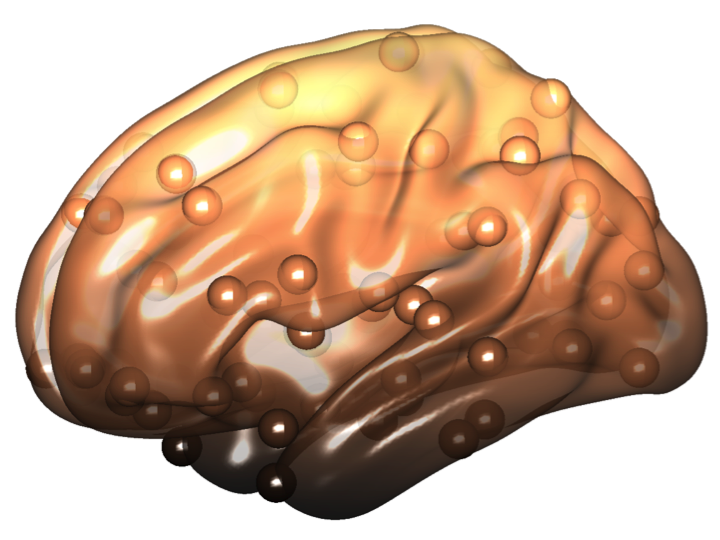
\includegraphics{tut_ba/fig01.png}}
	{Brain atlas figure created with BRAPH 2.0}
	{
	Example of a brain surface image with some nodes representing brain regions.
	}

\begin{abstract}
\noindent
This Tutorial explains how to work with the Graphical User Interface (GUI) to manage brain atlases.
This is typically the first step required to perform a graph analysis in BRAPH 2.0. 
In this Tutorial, we will explain you how to upload a brain atlas and how to visualize it.
\end{abstract}

\tableofcontents

\fig{figure*}
	{fig:02}
	{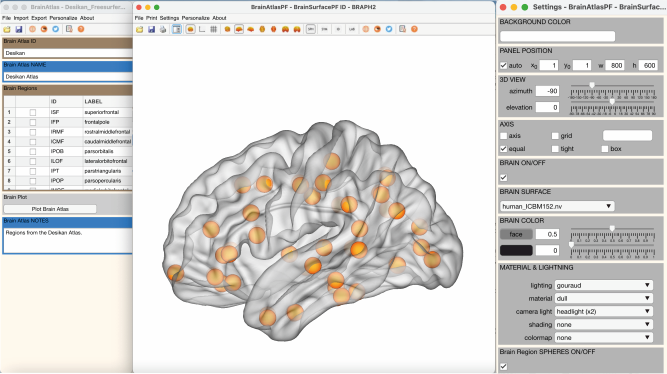
\includegraphics[height=10cm]{tut_ba/fig02.png}}
	{Brain Atlas GUI}
	{
	Full graphical user interface to work with a brain atlas in BRAPH 2.0. 
	}

\clearpage
\section{Open the GUI}

The brain atlas GUI is typically the first step in the BRAPH 2.0 pipelines. You can open it by typing braph2 in the MatLab's terminal, which allows you to select a pipeline containing the steps that you want to apply in your analysis. Once a pipeline has been selected, the first window will allow you to upload the brain atlas, as shown in \Figref{fig03}a.

\fig{figure*}
	{fig:03}
	{
	[h!]
	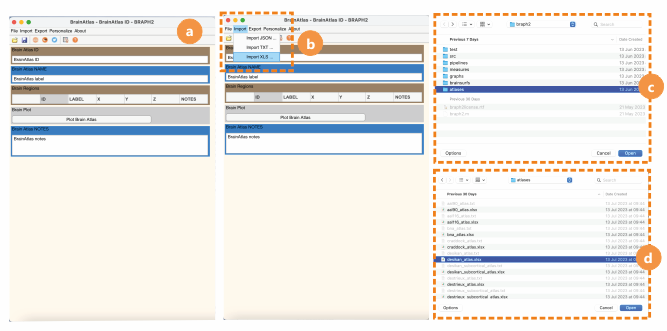
\includegraphics[height=10cm]{tut_ba/fig03.png}
	}
	{Upload a brain atlas}
	{
	The different steps you need to follow to open a brain atlas using the GUI. 
	}

To open the GUI and upload the brain atlas, you can also do it from the command line by typing the commands in \Coderef{cd:launch}.
%
\begin{lstlisting}[
	label=cd:launch,
	caption={
		{\bf Code to launch the Brain Atlas GUI.}
		This code can be used in the MatLab command line to launch the  Brain Atlas GUI.
	}
]
ba = BrainAtlas(); ¥\circled{1}\circlednote{1}{creates a new object \code{BrainAtlas}.}¥

gui = GUIElement('PE', ba); ¥\circled{2}\circlednote{2}{creates a GUI to upload the brain atlas.}¥
gui.get('DRAW') ¥\circled{3}\circlednote{3}{draws the GUI.}¥
gui.get('SHOW') ¥\circled{4}\circlednote{4}{shows the GUI.}¥
\end{lstlisting}

\section{Upload the Brain Atlas}

In this window opened in the previous step (a) you have a menu that you can use to import a brain atlas (b) that you created or has already been prepared for you to use from the atlases folder of BRAPH 2.0 (c). In this example, we are uploading the Desikan atlas (4) \Figref{fig3} . 
	
\fig{figure*}
	{fig:04}
	{
	[h!]
	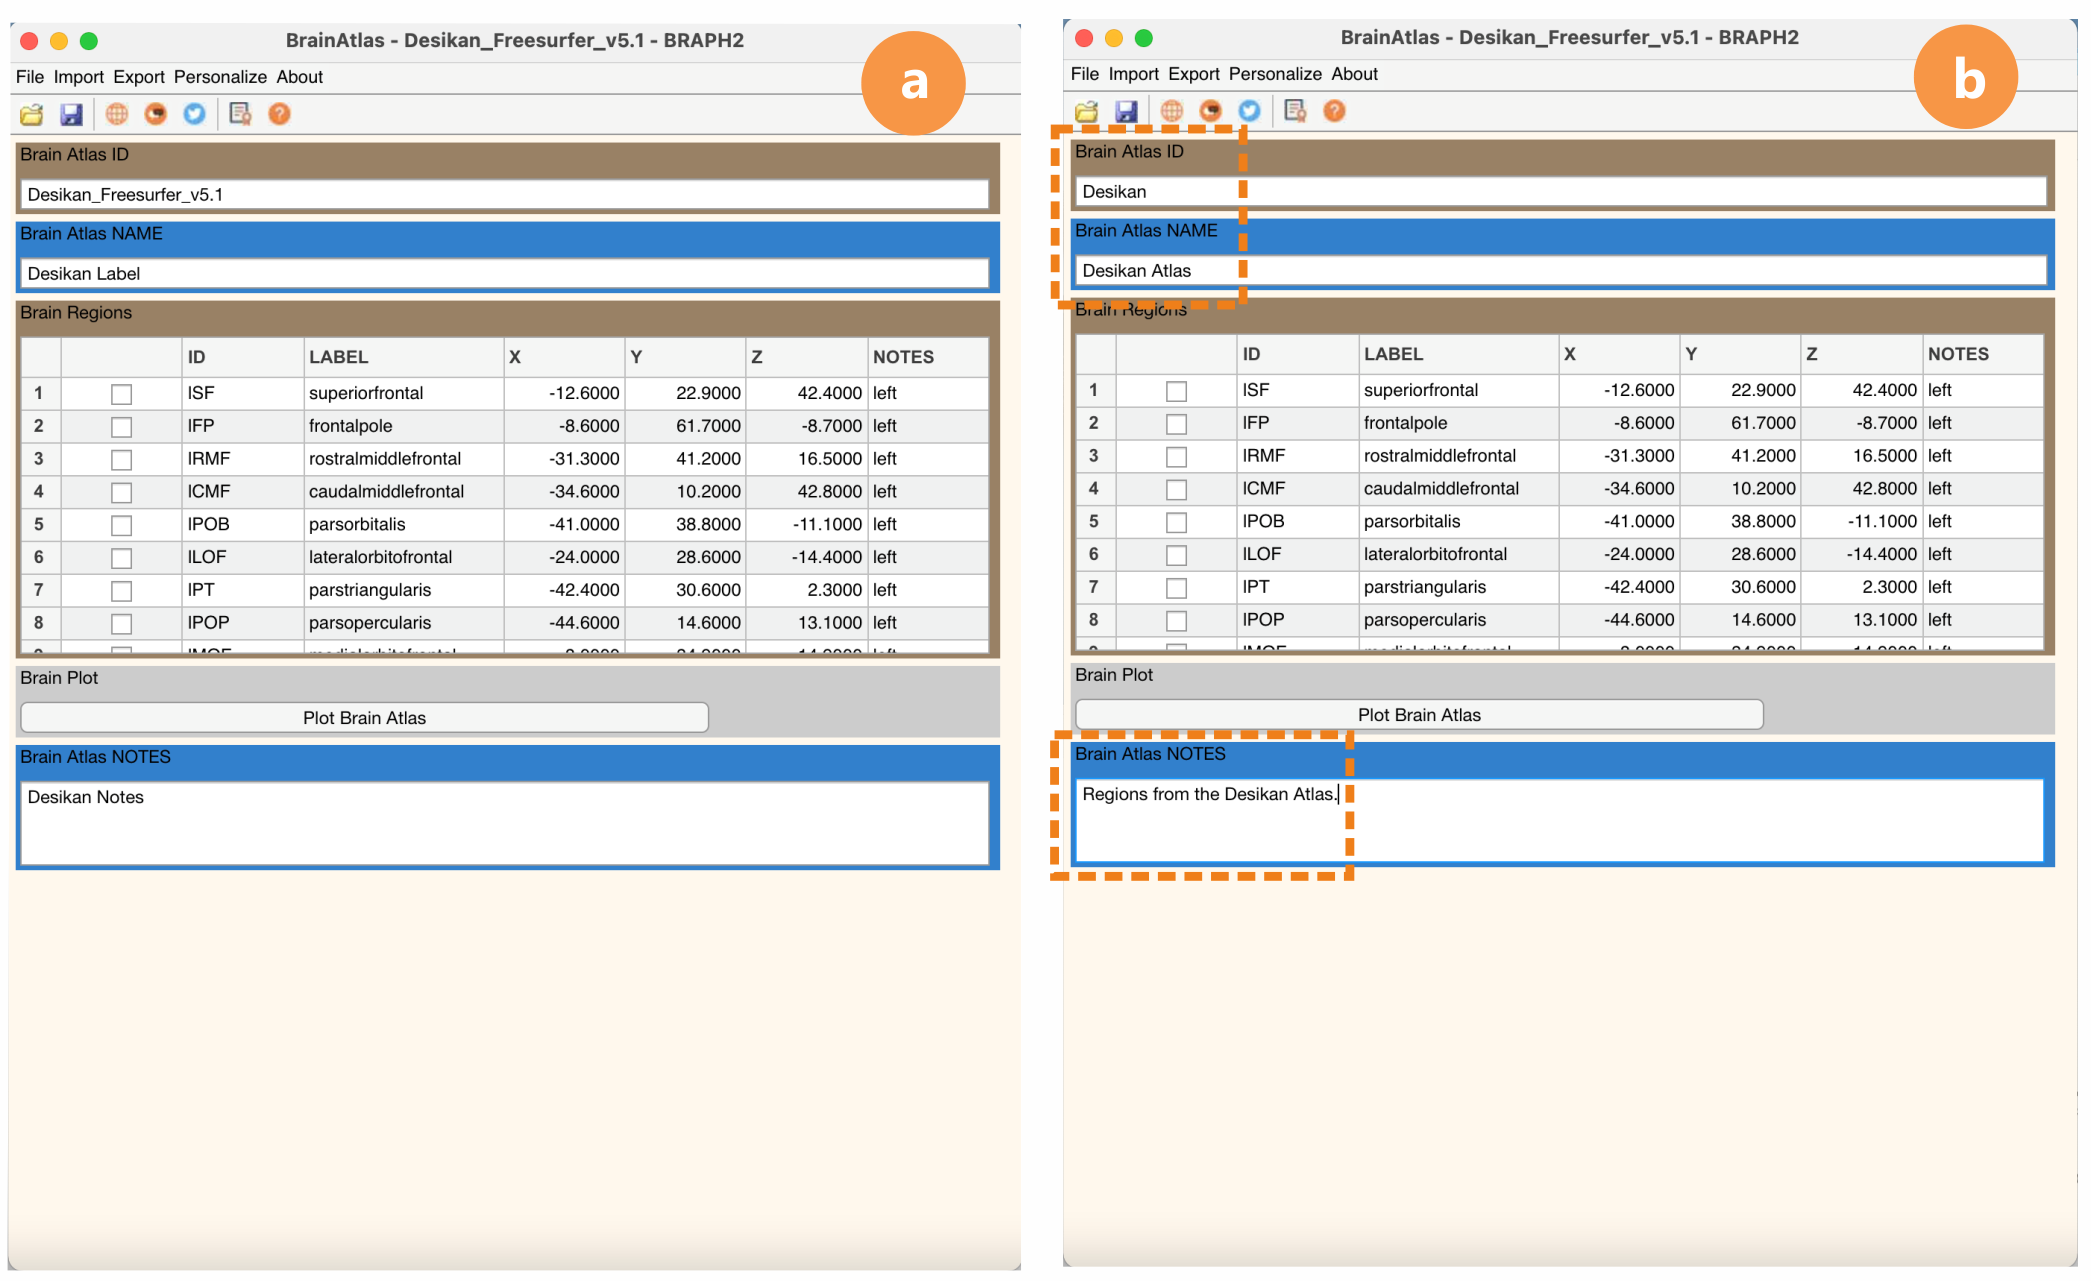
\includegraphics{tut_ba/fig04.png}
	}
	{Edit the atlas information}
	{
	A few examples of information that can be changed in the brain atlas GUI. 
	}

Note that you can change information in this GUI \Figref{fig4}a such as the brain atlas ID, the brain atlas name, the brain atlas description (2) as well as the IDs, labels, coordinates and notes of the brain regions \Figref{fig4}b .

\clearpage
\section{Ready Brain Atlases}

\fig{figure}
	{fig:05}
	{
	[b!]
	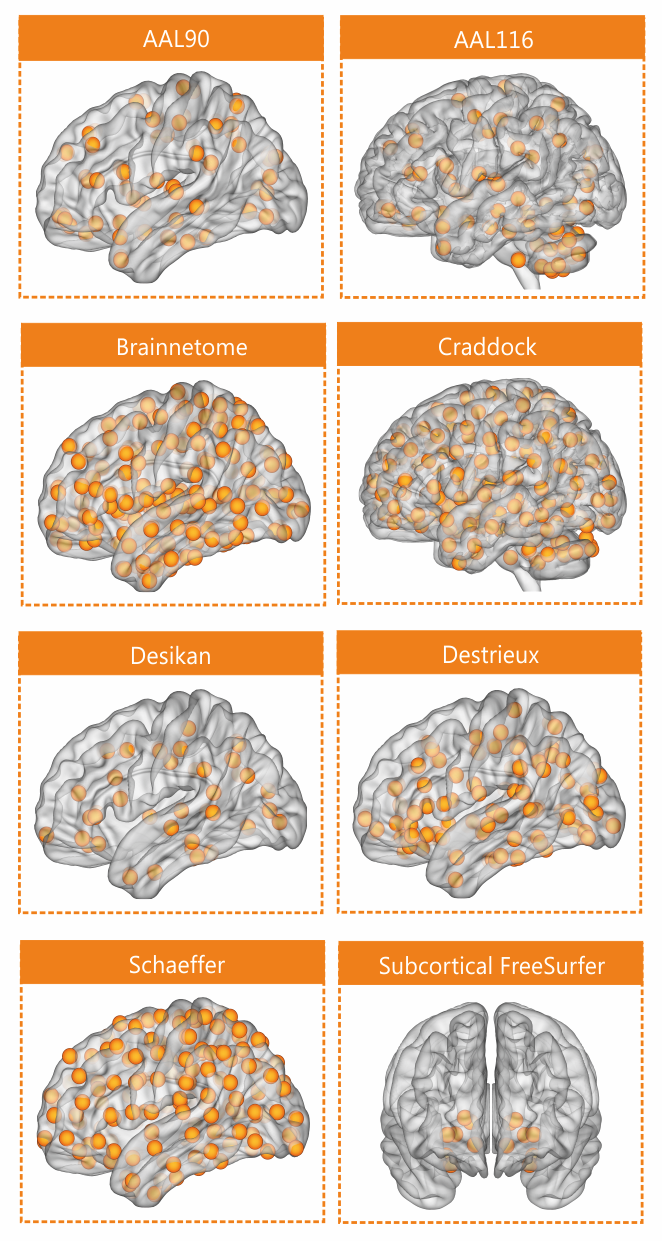
\includegraphics[height=15cm]{tut_ba/fig05.png}
	}
	{Brain Atlases}
	{
	Different brain atlases provided by BRAPH 2.0: \\
	{\bf AAL90} Automated Anatomical Labelling atlas with 90 cortical and subcortical regions.\\
	{\bf AAL116} Automated Anatomical Labelling atlas with 116 cortical and subcortical regions, including cerebellar areas.\\
	{\bf BNA} Brainnetome atlas with 246 cortical and subcortical regions.\\
	{\bf Craddock} Functional atlas with 200 cortical and subcortical regions, including cerebellar areas.\\
	{\bf Desikan} Anatomical atlas with 68 cortical from the FreeSurfer software.\\
	{\bf Destrieux} Anatomical atlas with 148 cortical from the FreeSurfer software.\\
	{\bf Schaefer} Functional brain atlas with 200 cortical regions that belong to 7 different resting-state fMRI networks.\\
	{\bf Subcortical FreeSurfer} Anatomical atlas with 14 subcortical gray matter regions from the FreeSurfer software.
	}

Currently, we provide several brain atlases that are commonly used in the field of brain connectomics, which can be downloaded from our website (\url{http://braph.org/software/brain-atlases/}) \Figref{fig5}.

\clearpage
\section{Create a New Brain Atlas}

To prepare a Brain Atlas in BRAPH 2.0 format, you should create a new excel file (.xls or .xlsx), as shown in \Figref{fig6}. 

\fig{figure}
	{fig:06}
	{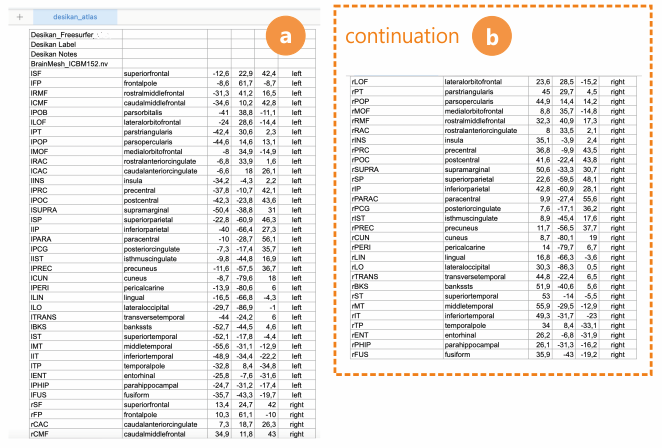
\includegraphics[height=10cm]{tut_ba/fig06.png}}
	{Preparing your own atlas}
	{
	Overview of how the excel file containing your atlas information should look like.  
	}

Start by writing the following information in the first 4 rows:
\begin{itemize}

\item Brain Atlas ID (row 1, column 1). 
For example: Desikan FreeSurfer v5.1

\item Brain Atlas LABEL (row 2, column 1). 
For example: Desikan Labels

\item Brain Atlas NOTES (row 3, column 1).
For example: Desikan Nodes

\item Brain Surface Name (row 4, column 1).
For example: BrainMeshICBM152.nv

\end{itemize}
Then, from row 5, you should include the IDs of the regions of your atlas (1st column), the Labels of the regions of your atlas (2nd column), the X, Y and Z coordinates (3rd, 4th and 5th columns) and the brain hemisphere or any notes you would like to add (6th column).	

\clearpage
\section{Plot the Brain Atlas}

Once you are satisfied you can plot your brain atlas (a), which will open a brain surface that contains the nodes corresponding to brain regions (b) \Figref{fig7}.

\fig{figure*}
	{fig:07}
	{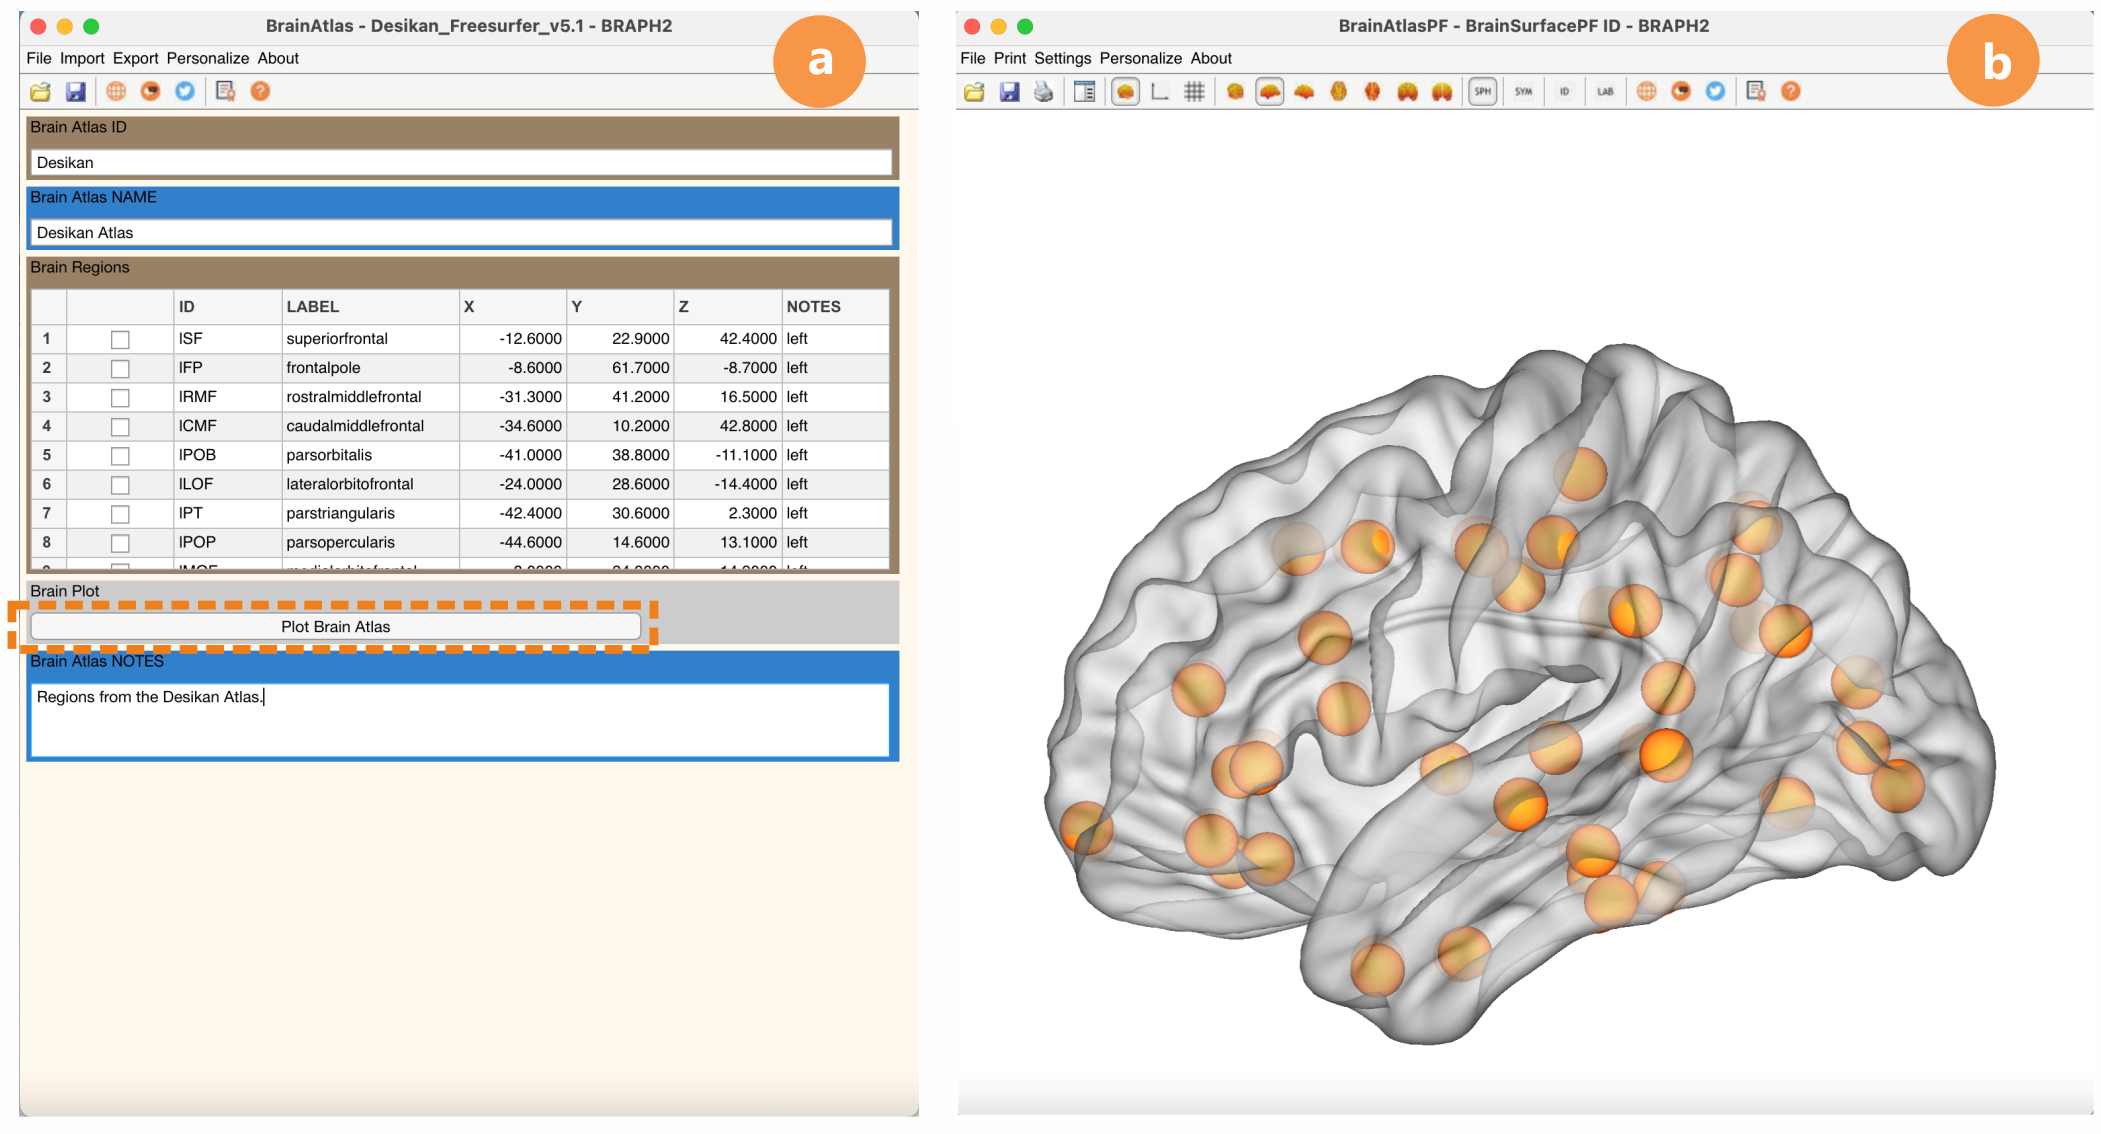
\includegraphics[height=10cm]{tut_ba/fig07.png}}
	{Brain atlas visualization.}
	{
	Plotting the nodes of a brain atlas on a 3D brain surface. 
	}
	
This new window has a large menu that allows you to change the visualization of the atlas. We suggest you try the different options to understand how they change the figure. Importantly, within this menu there is one option called Settings Brain Surface (a) which, when selected, will open another window, as can be seen below \Figref{fig8}.

\fig{figure*}
	{fig:08}
	{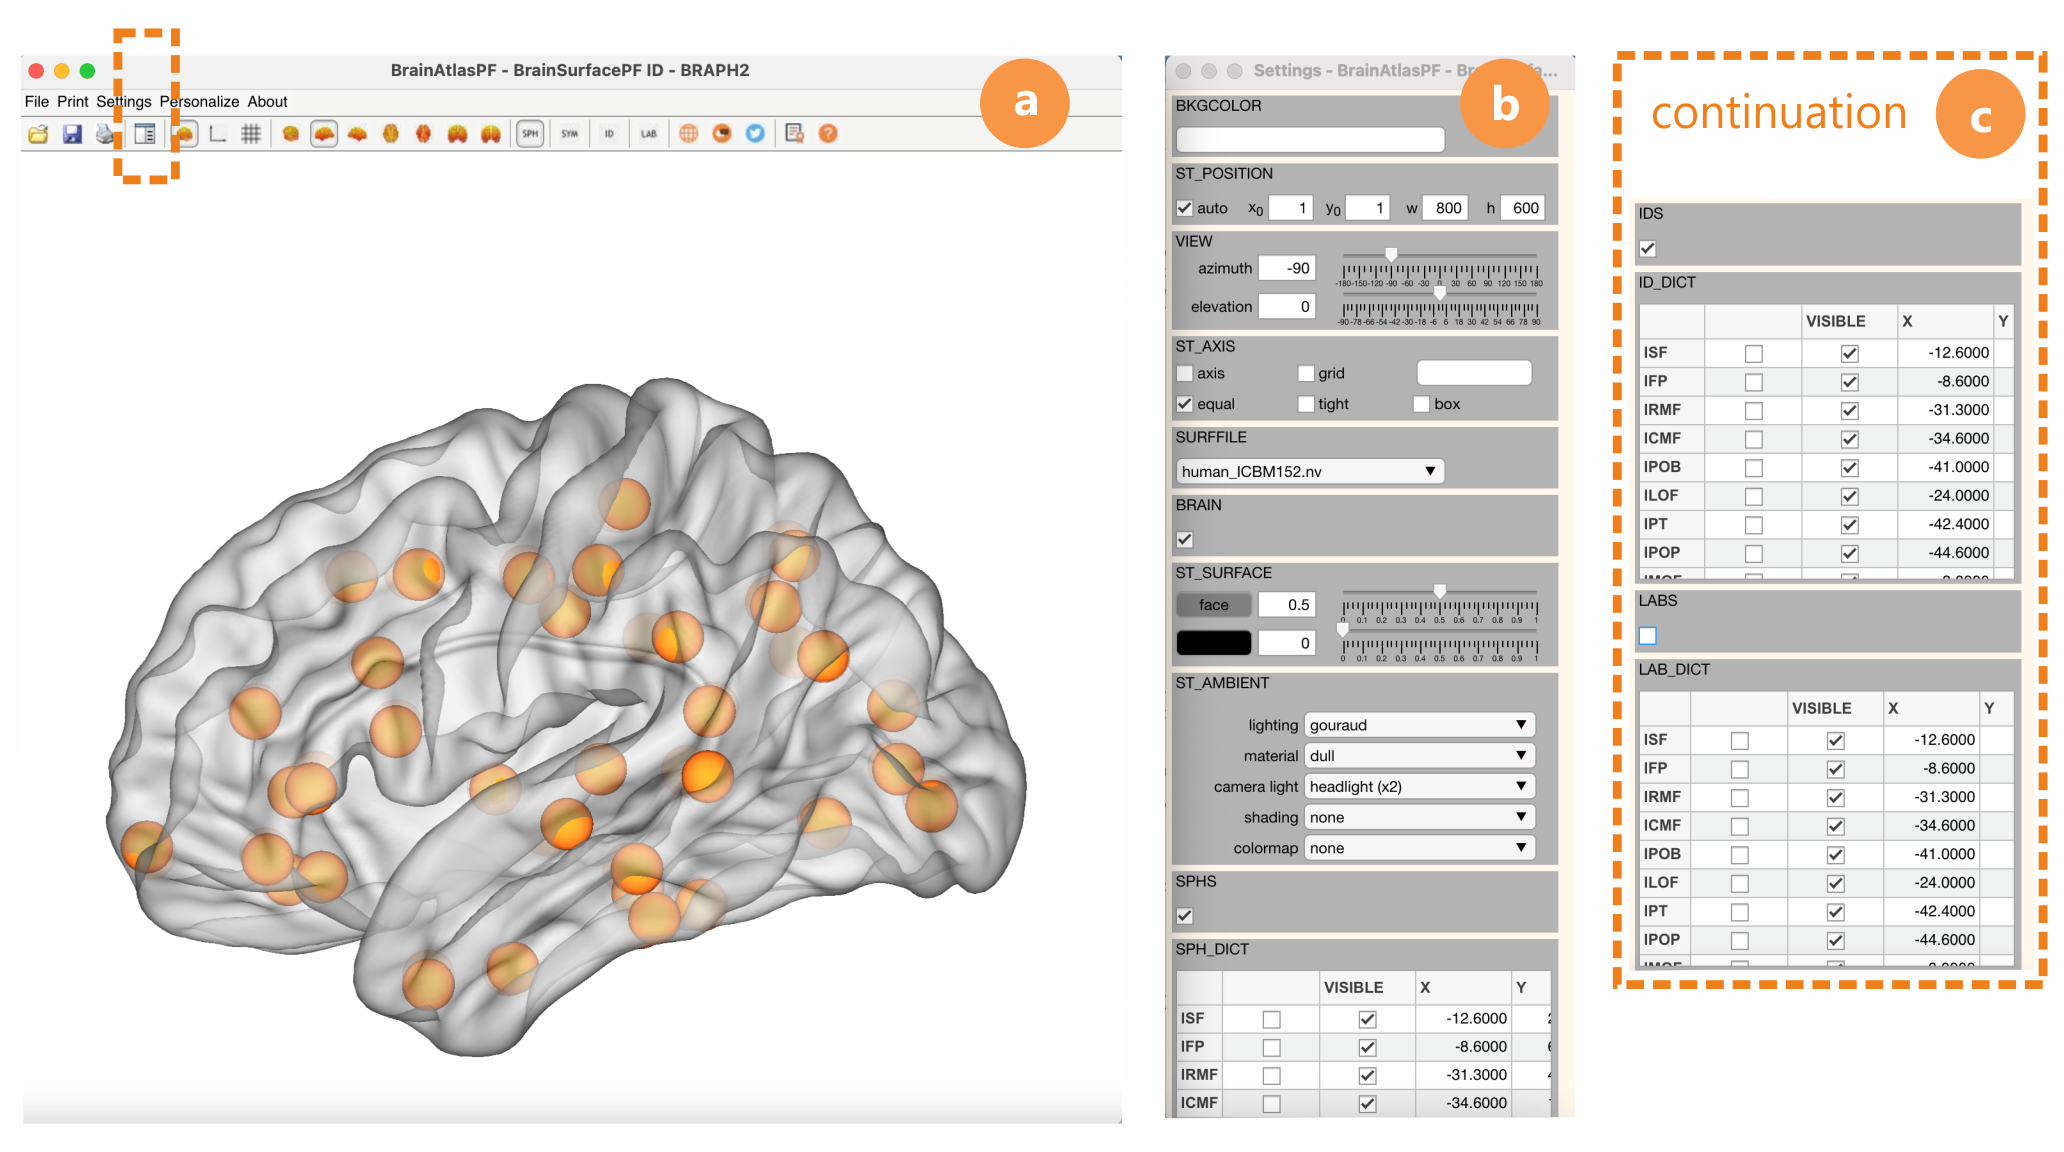
\includegraphics[height=10cm]{tut_ba/fig08.png}}
	{Visualization of brain atlas}
	{
	Changing the visualization of the brain atlas. 
	}

This window allows you to change different options (b, c), which are important to create a final figure with all the nodes included in your analysis, which is often included within the 1st figure of a manuscript.

Most things in this panel are intuitive and again we suggest that you try different options until you achieve the visualization you want.
Some things that might not be intuitive is the difference between spheres and symbols (the first one is the geometrical structure of a node, whereas the second is just a dot inside the sphere that denotes the presence of a region). 

If you wish to change the size of the spheres of all nodes, you need to right click and "select all" nodes in the first column, change the size of one node and right click to select "apply to selection".

The same applies if you want to change the colour of all nodes in the FACECOLOR column. Here the colors correspond to the hexadecimal form of RGB colors, which can be found online.

There are many possibilities for visualization. Here is just one example:

\fig{figure*}
	{fig:09}
	{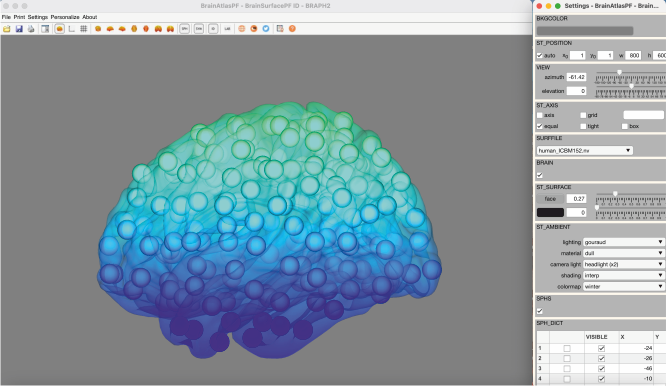
\includegraphics[height=10cm]{tut_ba/fig09.png}}
	{Example of a visualization of the brain atlas}
	{
	A final figure created with BRAPH 2.0 by changing different options in the menu.
	}

Importantly, BRAPH 2.0 provides different brain surfaces as shown in \Figref{fig10} for the human brain and cerebellum in addition to animals such as the ferret, macaque, mouse or rat.

\fig{figure*}
	{fig:10}
	{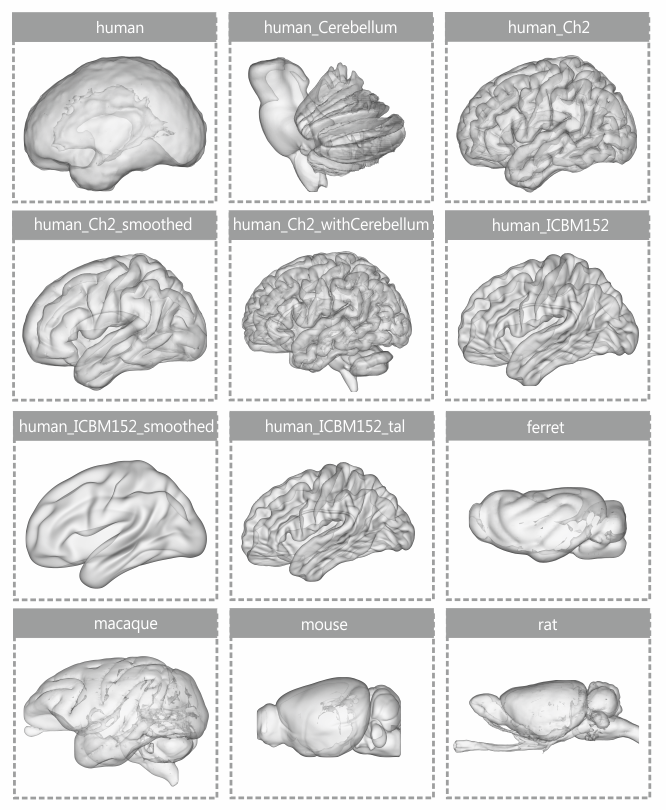
\includegraphics[height=10cm]{tut_ba/fig10.png}}
	{Brain surfaces in BRAPH 2.0}
	{
	Different brain surfaces that are available in BRAPH 2.0 to plot the brain atlas.
	}

\clearpage
\section{Export the Figure}

To export and save a figure, you can select print from the brain atlas GUI and select one of the various options we provide \Figref{fig11}.

\fig{figure*}
	{fig:11}
	{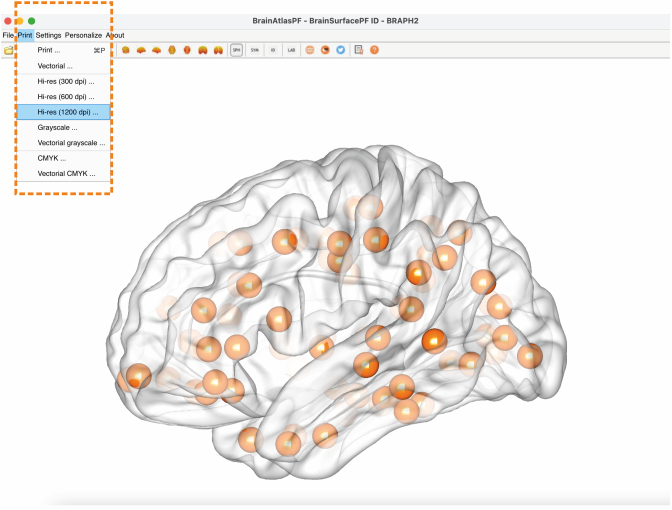
\includegraphics[height=10cm]{tut_ba/fig11.png}}
	{Saving a brain atlas figure}
	{
	We provide different options that allow saving a figure with different resolutions and colour modes. 
	}

\end{document}